%\documentclass{article}
%%%% Packages from Ben
\usepackage[backend=biber, style=nature, autocite=superscript, natbib=true]{biblatex}
\usepackage{enumitem}

%%% Packages . %from template
\usepackage{amsmath}
\usepackage{amstext}
\usepackage{amssymb}
\usepackage{graphicx}
\usepackage{import}
\usepackage[titletoc]{appendix}
\usepackage{lscape}

%%% Packages. %from TiN
\usepackage{comment}
\usepackage[T1]{fontenc}
%# \usepackage[latin9]{inputenc}
\usepackage{amstext}
\usepackage{graphicx}
\usepackage{amssymb}
\usepackage{multirow}
\usepackage{amsmath,amssymb}
\makeatletter
\makeatother
\usepackage{setspace}

%%% Packages from Dielectric loss
\usepackage{epsf}
\usepackage[T1]{fontenc}
\usepackage[utf8]{inputenc}
\usepackage{amstext}
\usepackage{graphicx}
\usepackage{amssymb}
\usepackage{multirow}
%\usepackage{multicol}
\usepackage{commath}
\usepackage{amsmath,amssymb}
%\usepackage{amslatex} %#
\usepackage{verbatim}
\makeatletter
\makeatother
\usepackage{comment}
%\usepackage{setspace}
%\doublespacing

%%% packages from xiy_notes, manybody_ramsey analog control writeup.
\usepackage[T1]{fontenc}
%\usepackage[latin9]{inputenc}
\usepackage[utf8]{inputenc}
\usepackage{amstext}
\usepackage{graphicx}
\usepackage{amssymb}
\usepackage{multirow}
\usepackage{amsmath,amssymb}
\usepackage{verbatim}
\usepackage{braket}
%\usepackage{float}
%\pagestyle{empty}
\usepackage{mathtools}

%%% Noise
%% Noise cal bias t
\usepackage[T1]{fontenc}
%\usepackage[utf8]{inputenc}
\usepackage{amstext}
\usepackage{amsmath}
\usepackage{amssymb}
\usepackage{graphicx}
\usepackage{tikz}
\usepackage{circuitikz}
\tikzstyle{densely dashed}=[dash pattern=on 4pt off 3pt]
\usepackage{verbatim}
\usepackage{float}

%MBL
\usepackage[T1]{fontenc}
\usepackage[utf8]{inputenc}
\usepackage{amstext}
\usepackage{graphicx}
%\usepackage[usenames, dvipsnames,hyperref]{xcolor} %from mk
%\usepackage{xcolor}
\usepackage{multirow}
\usepackage{amsmath,amssymb}
\usepackage{adjustbox}
\usepackage{verbatim}
\usepackage{braket}
\usepackage{mathtools}
\usepackage{rotating}
\usepackage{afterpage}
\usepackage[section]{placeins}
\usepackage{wrapfig}%
\usepackage{multicol}
\usepackage{caption}
\usepackage{setspace}
\usepackage[all]{nowidow}
\usepackage{subfiles}
\usepackage{lineno}
\usepackage[italic]{mathastext}
\usepackage{isomath}

% Packages from MBL main submitted:
\usepackage[all]{nowidow}
\usepackage{amssymb}
\usepackage{graphicx}
\usepackage{etoolbox}
\usepackage{scrextend}
\makeatletter
\newcommand{\lyxdot}{.}
\DeclareMathAlphabet{\mathpzc}{OT1}{pzc}{m}{it}
\usepackage{comment}
\usepackage{verbatim}
\usepackage{amsmath}
\usepackage{mathtools}
\usepackage{xfrac}
\usepackage{bm}
%\usepackage{xcolor}
%\usepackage{color}
%\usepackage{sectsty}
\definecolor{red}{rgb}{1,0,0}
\definecolor{green}{rgb}{0,1,0}
\definecolor{blue}{rgb}{0,0,1}
\definecolor{c1}{rgb}{0.178,0.63,0.17}
\definecolor{c2}{rgb}{0.09,0.740,0.81}
\definecolor{c3}{rgb}{0.12,0.46,0.7}
\definecolor{c4}{rgb}{0.58,0.40,0.74}
%\chapterfont{\color{blue}}
%\sectionfont{\color{blue}}
\let\saved@includegraphics\includegraphics
\AtBeginDocument{\let\includegraphics\saved@includegraphics}
\renewenvironment*{figure}{\@float{figure}}{\end@float}
%\newcommand{\psection}[1]{\textcolor{BLUE}{\textbf{\emph{#1}}}}
%\newcommand{\esection}[1]{\textcolor{GREEN}{\textbf{\emph{#1}}}}
%\newcommand{\preff}[1]{\textcolor{light-gray}{[#1]}}
%\newcommand{\pref}[1]{\textcolor{cyan}{[#1]}}
\newcommand{\schrodinger}{Schr\"{o}dinger}


% Packages from MBL_Submitted_Supplement
\renewcommand{\thefigure}{\textbf{S\arabic{figure}}}
\usepackage{mathrsfs}
\usepackage{fullpage}
\usepackage{amssymb}
\usepackage{graphicx}
\usepackage{amsmath}
\usepackage[strict]{changepage}
\usepackage{framed}
\usepackage{amsthm}
\usepackage{bbm}
\usepackage{colortbl}
\usepackage{epsfig}

\sloppy
% Ben

%\usepackage[margin=1.0in]{geometry}
\usepackage{amstext,amsmath,amssymb}
\usepackage{verbatim}
\usepackage{mathtools}
\usepackage{afterpage}
%\usepackage{authblk}
\usepackage[all]{nowidow}

\usepackage{subfiles}
\usepackage{titlesec}
\usepackage[labelfont=bf]{caption}

\DeclareMathOperator{\diag}{diag}
\DeclareMathOperator{\Tr}{\mbox{Tr}}
\DeclareMathOperator{\tr}{\mbox{tr}}
\DeclareMathOperator{\re}{\mbox{Re}}
\DeclareMathOperator{\im}{\mbox{Im}}
\DeclareMathOperator{\erfc}{{erfc}}
\DeclareMathOperator{\sign}{{sign}}

%\let\Oldsection\section
%\renewcommand{\section}{\FloatBarrier\Oldsection}

\let\Oldsubsection\subsection
\renewcommand{\subsection}{\FloatBarrier\Oldsubsection}

%\let\Oldsubsubsection\subsubsection
%\renewcommand{\subsubsection}{\FloatBarrier\Oldsubsubsection}

%%%
%\makeatletter
%\AtBeginDocument{% This is supposed to place a float barrier after each subsection.
  %\expandafter\renewcommand\expandafter\subsection\expandafter{%
    %\expandafter\@fb@secFB\subsection
  %}%
%}
%\makeatother
\usepackage[titletoc]{appendix}
%%\newcommand{\bra}[1]{\langle #1 |}
%\newcommand{\ket}[1]{| #1 \rangle }
%\newcommand{\braket}[2]{\langle #1|#2\rangle}
%\newcommand{\bbraket}[3]{ \langle #1 | #2 | #3 \rangle }
%\newcommand{\norm}[1]{\| #1\|}

% noise cal bias t

%\renewcommand{\Re}{\textrm{Re}}
%\renewcommand{\Im}{\textrm{Im}}
% Figures. Example usage:
% \quickfig{\columnwidth}{my_image}{This is the caption}{fig:my_fig}
\DeclareRobustCommand{\quickfig}[4]{
\begin{figure}
    \begin{centering}
        \includegraphics[width=#1]{#2}
        \par\end{centering}
    \caption{#3}
    \label{#4}
\end{figure}
}

\DeclareRobustCommand{\quickwidefig}[4]{
\begin{figure*}[h]
    \begin{centering}
        \includegraphics[width=#1]{#2}
        \par\end{centering}
    \caption{#3}
    \label{#4}
\end{figure*}
}

% From MBL work
\newcommand{\bc}[1]{{\color{RoyalBlue}#1}}
%\newcommand{\bc}[1]{{\color{RoyalBlue} MK: #1}}
\newcommand{\bcch}[1]{{\color{OliveGreen} #1}}
\newcommand{\bcrd}[1]{{\color{BrickRed} BC: #1}}
\newcommand{\nqninet}{N_{q_\text{9}} \left( t \right)}
%\renewcommand{\familydefault}{\sfdefault}
%\usepackage{helvet}

%\makeatletter
%\def\@maketitle{%
%\newpage
%\null
%\vskip 2em%
%\centering
%\let \footnote \thanks
%{\LARGE \@title \par}%
%\vskip 1.5em%
%{\large
%\lineskip .5em%
%\begin{tabular}[t]{c}%
    %\baselineskip=12pt
    %\@author
%\end{tabular}\par}%
%\vskip 1em%
%{\large \@date}%
%\par
%\vskip 1.5em}
%\makeatother


%\setcounter{topnumber}{2} %  maximum number of floats in the top area
%\setcounter{bottomnumber}{2} % maximum number of floats in the bottom area
%\setcounter{totalnumber}{4} % maximum number of floats on a text page
%\renewcommand{\topfraction}{0.99} % The maximum size of the top area
%\renewcommand{\bottomfraction}{0.99} %The maximum size of the bottom area
%\renewcommand{\textfraction}{0} %  The area that must not be occupied by floats
%\renewcommand{\floatpagefraction}{0.999} % the minimum part of the page that need to be occupied by floats to for a float page
%\setlength{\floatsep}{5pt plus 2pt minus 2pt}  % The separation between floats in the top and bottom areas
%\setlength{\textfloatsep}{5pt plus 2pt minus 2pt} % The separation between the top or bottom area and the text area
%\setlength{\intextsep}{5pt plus 2pt minus 2pt}  % For inline floats (placed by "here")

%\setstretch{1.0}
%\setlength{\columnwidth}{225 pt}
%\setlength{\columnsep}{20 pt}
%\small

%\title{Bias-T Specification for Noise Spectra Calibration}
%\author{B. Chiaro\\\small{Department of Physics, University of California, Santa Barbara, California 93106, USA}}
%\date{\today}

%\begin{document}

%\maketitle

%\begin{abstract}
We show the basic circuit analysis and the physical implementation for the Bias T that we use for the noise spectra calibration.  We use a SPICE simulation to check that this circuit will work up to at least 100\,MHz.
%\end{abstract}

\section{Schematic}

We know from experiments that the calibration works well when the Agillent AWG outputs a 5V sin wave through a 70db attenuator to the qubit.
Here we design a bias-T that gives 70 dB power attenuation between the AWG and the qubit using voltage division.  

The schematic for the bias T is shown in Fig,\,\ref{fig.circuit_diagram}.
The circuit as seen by the AWG is shown in Fig.\,\ref{fig.circuit_as_seen_by_awg}.

\begin{figure}[ht]
\begin{centering}
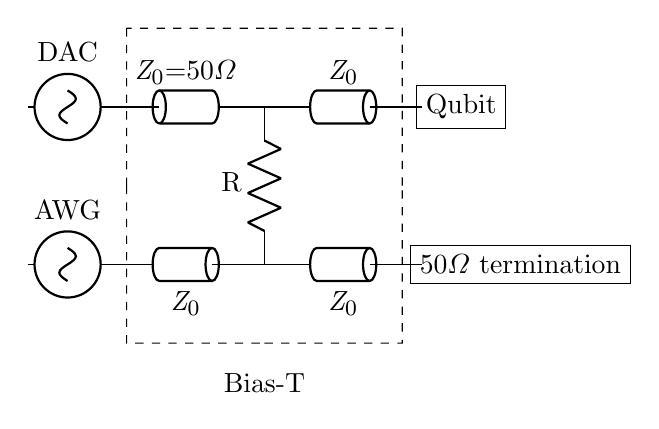
\begin{tikzpicture}
\draw (-1,2)
to [vsourcesin,l=$\text{DAC}$] (0,2);
\draw (-1,0)
to [vsourcesin,l=$\text{AWG}$] (0,0);
\draw (0,0)
to [TL,l_=$Z_{0}$] (2,0)
to [R=$\text{R}$] (2,2)
to [TL,l_=$Z_{0} \text{=} 50 \Omega$] (0,2);
\draw (2,0)
to [TL,l_=$Z_{0}$] (4,0);
\draw (2,2)
to [TL,l^=$Z_{0}$] (4,2);
\node[draw,align=left] at (5.25,0) {$50 \Omega$ termination};
\node[draw,align=left] at (4.5,2) {Qubit};
% box around bias-T
\draw[dashed] (0.25,3)
to [short] (0.25,-1)
to [short] (3.75,-1)
to [short] (3.75,3)
to [short] (0.25,3);
\node at (2,-1.5) {Bias-T};
\end{tikzpicture}
\par\end{centering}
\caption{Diagram of the tee circuit.}
\label{fig.circuit_diagram}
\end{figure}

\begin{figure}[ht]
\begin{centering}
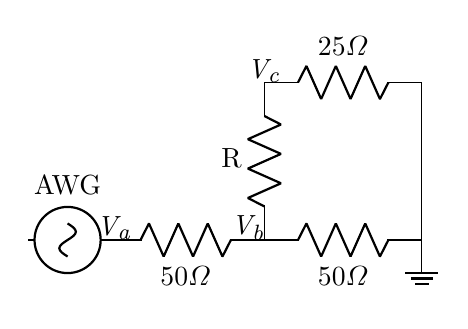
\begin{tikzpicture}
\draw (-1,0)
to [vsourcesin,l=$\text{AWG}$] (0,0);
\draw (0,0)
to [R,l_=$\text{50}\Omega$] (2,0)
to [R=$\text{R}$] (2,2)
to [R,l^=$\text{25}\Omega$] (4,2)
to [short] (4,0);
\draw (2,0)
to [R,l_=$\text{50}\Omega$] (4,0)
to [short] node[ground] {} (4,0);
\draw (0.1,0.15) node[circle] {$V_a$};
\draw (1.8,.15) node[circle] {$V_b$};
\draw (2,2.15) node[circle] {$V_c$};
\end{tikzpicture}
\par\end{centering}
\caption{Circuit as seen by the AWG.}
\label{fig.circuit_as_seen_by_awg}
\end{figure}

The condition on the resistor R (to get 70\,dB attn)  is
\begin{align}
70 &= 20 \log_{10}\left({\frac{V_a}{V_c}}\right) \\
\frac{10^{3.5}}{2} &= \frac{V_b}{V_c} \, .
\end{align}
From the divider equation
\begin{align}
V_c &= V_b \frac{25}{R + 25} \\
R &= \frac{25}{2}10^{3.5} - 25 = 39.5 \, \text{K} \Omega \, .
\end{align}

We should check how much current will go to the DAC assuming $\text{V}_a = 5 \, \text{V}$.
The current going to the DAC is $\frac{1}{2} \left( 2.5 \, V / 39.5 \, \text{K} \Omega \right) = 32 \, \mu A$, since half of the current across R goes to the DAC.

To get a crude idea if we need to worry about microwave problems we calculate the on-chip wavelength at 100\,MHz assuming $\epsilon_{\text{substrate}} = 4.6$:
\begin{equation}
\epsilon_{r} = (1+\epsilon_{\text{substrate}})/2 = 2.8\,\epsilon_0 \, .
\end{equation}
The propagation velocity on board is $c/\sqrt{\epsilon_r} = 1.8 \times 10^8$ m/sec.
So our 100 MHz signal has a wavelength of 1.8\,m.
This should be fine, we'll just make the board small.

\begin{comment}
To check how "Microwavy" The board needs to be lets calculate the wavelength at 100 MHz which is roughly the high end of the range that we wish to calibrate.  Since we build the board out of FR4 which has $\epsilon$=4.6 our $\epsilon_{r}$ is (1+4.6)/2 = 2.8 $\epsilon_0$.

In typical operation port 4 of the device is 50 $\Omega$ terminated.

\begin{figure}[ht]
\begin{center}
\begin{circuitikz}
\draw (-1,2)
to [vsourcesin,l=$\text{DAC}$] (0,2);
\draw (-1,0)
to [vsourcesin,l=$\text{Agilent}$] (0,0);
\draw (0,0)
to [TL,l_=$Z_{0}$] (2,0)
to [R=$\text{75 K}\Omega$] (2,2)
to [TL,l_=$Z_{0} \text{=} 50 \Omega$] (0,2);
\draw (2,0)
to [R,l_=$50 \Omega$] (4,0)
to [short] node[ground] {} (5,0);
\draw (2,2)
to [TL,l_=$Z_{0}$] (4,2);
\end{circuitikz}
\end{center}
\end{figure}
\end{comment}

\section{Physical Implementation}

\quickfig{\columnwidth}
{NoiseCalBiasT_PCB_Drawing1.png}
{
The PCB layout for the bias-T.
Red is the top metal of the circuit, grey are through vias to the back side metal.
The back side metal (blue) is a continuous ground plane}
{fig.pcb}

The physical layout of the board is shown in Fig.\,\ref{fig.pcb}.
The geometry of the transmission line is a GCPW.
I'm assuming a board thickness of .062 mil = 1.57 mm since this is compatible with the 50\,$\Omega$ connector that we often use in the lab (Johnson Components \#: 142-0701-801).

For the transmission line parameters in the spice model I got $Z_0$ and $\epsilon_{relative}$ from the online calculator for the gcpw at http://chemandy.com/calculators/coplanar-waveguide-with-ground-calculator.htm.
I used the following parameters:
\begin{itemize}
\item $\epsilon_{\text{substrate}} = 4.6$
\item $\text{track width} = 1.2\,\text{mm}$
\item $\text{gap width} = 0.2\,\text{mm}$
\item $\text{board thickness} = 1.57\,\text{mm}$
\end{itemize}
This gave $\epsilon_{\text{eff}} = 2.879$ and characteristic impedance of  $50.16\,\Omega$.

\section{SPICE Simulation}
We perform a SPICE simulation to predict the maximum operating frequency for the calibration.

We convert the calculated $Z_0$ and $\epsilon_r$ to $L_l$ and $C_l$ since these are the inputs required by SPICE:
\begin{itemize}
\item $Z_0 = \sqrt{L_l / C_l}$
\item $\nu_p = 1/\sqrt{L_l C_l} = 1 / (\mu_0 \epsilon_r \epsilon_0) = \nu_c / \sqrt{\epsilon_r}$
\item $C_l = (Z_0 \nu_p)^{-1}$
\item $L_l = Z_0 / \nu_p$
\end{itemize}
For this geometry we have $L_l = 283\,\text{nH/m}$ and $C_l = .112\,\text{nF/m}$.
We plug these values into the SPICE schematic shown below in Fig.\,\ref{fig.SPICE_schematic}.

\quickfig{\columnwidth}
{NoiseCalBiasT_SPICE_Circuit1.png}
{
The bias-T SPICE simulation schematic, including the physical transmission line parameters from the layout.}
{fig.SPICE_schematic}

\quickfig{\columnwidth}
{NoiseCalBiasT_SPICE_Sim1.png}
{
The bias-T SPICE simulation results (with bad rendering) with a voltage probe across the qubit resistor R2.
This shows that at 100\,MHz the change in response is 0.01 dB.
There is less than 1\,dB change until above 700\,MHz.
We see that the DC calculation was well within our error tolerance for this part.}
{fig:SPICE_data}

To give a shorter stub connecting the P12 transmission line we move the resistor R asymmetrically toward that line.  We also add the parasitics of the capacitor to give a more realistic performance.

\quickfig{\columnwidth}
{NoiseCalBiasT_SPICE_Circuit2_parasitic.png}
{
Circuit model including asymmetric resistor placement and resistor parasitics}
{fig:SPICE_schematic_with_parasitics}

\quickfig{\columnwidth}
{NoiseCalBiasT_SPICE_Sim2_parasitic.png}
{
Circuit model including asymmetric resistor placement and resistor parasitics}
{fig:SPICE_results_with_parasitics}

We see that with the parasitics this part will not work up to 100 MHz.  We can achieve the performance that we want by reducing the Resistance and attenuating the source to give the desired output.  Reducing R to $10$\,$K\Omega$ is simulated below.

\quickfig{\columnwidth}
{NoiseCalBiasT_SPICE_Sim2_parasitic_10K.png}
{
Circuit model with 10K resistor including asymmetric resistor placement and resistor parasitics}
{fig:SPICE_results_with_parasitics}


\begin{comment}
To predict the maximum frequency of operation for this bias T were going to do a SPICE simulation of the circuit below where the parasitic capacitance is from a COMSOL simulation.
\end{comment}

% \end{document}